\documentclass[11pt]{article}
% \pagestyle{empty}

\setlength{\oddsidemargin}{-0.25 in}
\setlength{\evensidemargin}{-0.25 in}
\setlength{\topmargin}{-0.9 in}
\setlength{\textwidth}{7.0 in}
\setlength{\textheight}{9.0 in}
\setlength{\headsep}{0.75 in}
\setlength{\parindent}{0.3 in}
\setlength{\parskip}{0.1 in}
\usepackage{epsf}
\usepackage{pseudocode}
\usepackage{ amssymb }
\usepackage{mathtools}
\usepackage{amsmath}
\usepackage{tikz}
\usetikzlibrary{arrows}
\tikzset{
    vertex/.style={circle,draw,minimum size=1.5em},
    edge/.style={->,> = latex'}
}



\DeclarePairedDelimiter\ceil{\lceil}{\rceil}
\DeclarePairedDelimiter\floor{\lfloor}{\rfloor}

% \usepackage{times}
% \usepackage{mathptm}

\def\O{\mathop{\smash{O}}\nolimits}
\def\o{\mathop{\smash{o}}\nolimits}
\newcommand{\e}{{\rm e}}
\newcommand{\R}{{\bf R}}
\newcommand{\Z}{{\bf Z}}


\DeclareMathOperator*{\argmin}{arg\,min}
\DeclareMathOperator*{\argmax}{arg\,max}

\begin{document}

\title{CS 124 HW5}
\author{HUID: 90904116\\ %replace with your name
CS124 - Data Structures and Algorithms} 
\maketitle



\textit{For all homework problems where you are asked to give an algorithm, you must prove the correctness of your algorithm and establish the best upper bound that you can give for the running time. You should always write a clear informal description of your algorithm in English. You may also write pseudocode if you feel your informal explanation requires more precision and detail. As always, try to make your answers as clear and concise as possible.}

\begin{enumerate}

\item Assume there is a unique solution to E($P_i$), the expected number of moves to reach $n$ starting from position $i$ using random walk with a partially reflecting boundary. By definition, we know that E($P_n$) = 0, and from any position $0 \textless i \textless n$, E($P_i$) = 1 + $\frac{1}{2}$E($P_{i+1}$) + $\frac{1}{2}$E($P_{i-1}$). Finally, for our partially-reflecting boundary, we have E($P_0$) = 1 + $\frac{1}{2}$E($P_{1}$) + $\frac{1}{2}$E($P_{0}$).\\

Now, assume that E($P_i$) = $(n-i)(n+i+1)$. We must show that this close-form solution satisfies the above three conditions. \\
1) From position $n$, E($P_n$) = $(n-n)(n+n+1)= 0$ \\
2) From any position $0 \textless i \textless n$, E($P_i$) = 1 + $\frac{1}{2}$E($P_{i+1}$) + $\frac{1}{2}$E($P_{i-1}$) = 1 + $\frac{1}{2}(n-i-1)(n+i+2) + \frac{1}{2}(n-i+1)(n+i)$ =  1 + $\frac{1}{2}(n^2 - i^2 + n - 3i - 2) + \frac{1}{2}(n^2 + n - i^2 + i) = 1 + n^2 + n - i^2 - i - 1 = (n^2 - i^2) + (n-i) = (n+i)(n-i) + (n-i) = (n+i + 1)(n-i)$\\
3) starting from the reflecting boundary, E($P_0$) = 1 + $\frac{1}{2}$E($P_{1}$) + $\frac{1}{2}$E($P_{0}$) = 1 + $\frac{1}{2} (n-1)(n+2) + \frac{1}{2} n(n+1) = 1 + n^2 + n - 1 = n^2 + n = n(n+1)$, which satisfies $(n-i)(n+i+1)$ when $i=0$

As we can see, our close-form solution E($P_i$) = $(n-i)(n+i+1)$ satisfies our three necessary conditions for a reflecting boundary and the expected number of steps to reach $n$ from position $i$, with $i \in \Z; 0 \leq i \leq n$, is E($P_i$) = $(n-i)(n+i+1)$. 

\newpage
\item 
\includegraphics[angle=270,scale=.15]{pic1}

\newpage
Step 3: DFS from $s$ to $t$ (s-c-d-t) \\
Current flow from $s$ to $t$: 7 \\
residual graph (3): \\
\includegraphics[angle=90, scale=.15]{pic2}

While their still exist reverse edges $(v,u)$ = c(u,v) - $f_{uv}$ for all edges $(u,v)$ with positive flow going through them, my algorithm has run out of paths from $s$ to $t$. Therefore, we conclude that the maximum flow from $s$ to $t$ is 8. The final cut is $S \setminus V$, with nodes reachable from $s$ are $S$ = [$s,a,c,d$]. Since the sum of edge weights crossing $S$ in our original graph $G$ is also 8, we are sure that the maximum flow is 8.


\newpage
\item First, determine capacity $C$, the number of subplots that support plant growth, of every row $r_1,r_2,...r_n$ and every column $c_1,c_2,...c_n$, where $0 \leq C(r_i) \leq n$ and $0 \leq C(c_i) \leq n$. While iterating through all rows and columns, keep track of the minimum capacity among all rows and columns \\ $m =$ min($C(r_1),...,C(r_n),...,C(c_1),...,C(c_n)$). Since there are one or more rows/columns with capacity $m$, we know $p$ cannot be greater than $m$. Now, consider the graph below:

\begin{tikzpicture} [scale=3]
\node[vertex] (1) at (0,0) {$s$};
\node[vertex] (2) at (1.5,1) {$r_1$};
\node[vertex] (3) at (1.5 ,0) {$r_2$};
\node[vertex] (4) at (1.5 ,-1) {$r_n$};

\node[vertex] (5) at (3,1) {$c_1$};
\node[vertex] (6) at (3 ,0) {$c_2$};
\node[vertex] (7) at (3 ,-1) {$c_n$};

\node[vertex] (8) at (4.5 ,0) {$t$};

\draw[edge] (1) -- (2) node[midway, above] {$m$};
\draw[edge] (1) -- (4) node[midway, above] {$m$};
\draw[edge] (1) -- (3) node[midway, above] {$m$};

\draw[edge] (2) -- (5) node[midway, above] {$1$};
\draw[edge] (2) -- (6) node[midway, above] {$1$};
\draw[edge] (2) -- (7) node[midway, below] {$1$};

\draw[edge] (3) -- (5) node[midway, below] {$1$};
\draw[edge] (3) -- (7) node[midway, above] {$1$};

\draw[edge] (4) -- (5) node[midway, above] {$1$};
\draw[edge] (4) -- (7) node[midway, above] {$1$};

\path (3) -- node[auto=false]{\ldots} (4);
\path (6) -- node[auto=false]{\ldots} (7);


\draw[edge] (5) -- (8) node[midway, above] {$m$};
\draw[edge] (6) -- (8) node[midway, above] {$m$};
\draw[edge] (7) -- (8) node[midway, above] {$m$};

\end{tikzpicture}

To represent this problem as a flow problem, we create a source with edges to each row $r_i$ with flow capacity $m$. Each row node has edges to the columns corresponding to entries in which it holds arable subplots. That is, for all fertile subplots $x_{ij}$ in our square plot, there exists edge $(r_i,c_j) \in G$. Finally, include edges from all column nodes to sink $t$ with capacity $m$. We limit flow capacity to $m$ on nodes emanating from $s$ and nodes leading into $t$ because there exist one or more rows or columns with farming capacity $m$ and all rows and columns must have an equal number of palm trees.\\

To find an arrangement of palm trees that maximizes $p$, we solve the max-flow linear program corresponding to $G$:

max $\sum f_{S,*}$ (maximize the sum of all flow leaving $S$)\\
for all nodes $w \in G; w \neq s,t$: $\sum_{(u,w)} f_{uw} - \sum_{(w,v)} f_{wv} = 0$ \\
for all edges $(u,v)$ in $G$: $0 \leq f_{uv} \leq c_{uv}$ (where $c_{uv}$ is the capacity of edge $(u,v) \in G$) \\
Since all rows and columns have capacity greater than or equal to $m$, we are guaranteed to find a solution with max-flow $n*m$ via our linear program. To find our solution after solving this program, we simply iterate through all rows $r_i$ in the max-flow graph and plant a tree at position ($i,k$) in our graph for all edges $(i,k)$ outgoing from $r_i$.

Run-time Analysis. Determining the minimum capacity $m$ requires iterating through all elements twice, via rows and columns, and takes O($2n$) = O($n$) time. By running the Edmonds-Karp Algorithm, a variation of Ford-Fulkerson with BFS, we can solve our linear program in time O($VE^2$), where $V=2n+2=O(n)$ and $E=2n+n^2=O(n^2)$. So the run-time of our flow-problem solver is O($VE^2$) = O($n*(n^2)^2$) = O($n^5$). Constructing our farm plot from the max plot takes time O($V + E$) = O($n^2$). So, overall, our algorithm takes run-time O($n$) + O($n^5$) +  O($n^2$) = O($n^5$)

\newpage
\item 1) In our max-flow problem in graph $G$ with source $s$ and sink $t$, we want to maximize flow subject to the following constraints: \\
max $\sum f_{S,*}$ (maximize the sum of all flow leaving $S$)\\
for all nodes $w \in G; w \neq s,t$: $\sum_{(u,w)} f_{uw} - \frac{1}{2} \sum_{(w,v)} f_{wv} = 0$ \\
for all edges $(u,v)$ in $G$: $0 \leq f_{uv} \leq c_{uv}$ (where $c_{uv}$ is the capacity of edge $(u,v) \in G$) \\
Then we solve the above problem via linear programming.

\vskip .3cm
2) First, ignore all edge costs $c_e$ in our graph $G$ and solve the max flow problem (same as above): \\
max $\sum f_{S,*}$ (maximize the sum of all flow leaving $S$)\\
for all nodes $w \in G; w \neq s,t$: $\sum_{(u,w)} f_{uw} - \sum_{(w,v)} f_{wv} = 0$ \\
for all edges $(u,v)$ in $G$: $0 \leq f_{uv} \leq c_{uv}$ (where $c_{uv}$ is the capacity of edge $(u,v) \in G$) \\
\vskip .04cm
To determine the max flow in our graph, we solve the above problem via linear programming. Once we determine $m$, the max-flow in $G$, we set up another linear program incorporating our max flow as a constraint and minimizing sum of all edge costs $c_e$ in our  graph: \\
min $\sum_{(u,v)} c_{uv} * f_{uv}$ (for all edges $(u,v) \in G$, multiply flow going through by cost to get total cost)\\
$\sum f_{S,*} = m$ \\
for all nodes $w \in G; w \neq s,t$: $\sum_{(u,w)} f_{uw} - \sum_{(w,v)} f_{wv} = 0$ \\
for all edges $(u,v)$ in $G$: $0 \leq f_{uv} \leq c_{uv}$ (where $c_{uv}$ is the capacity of edge $(u,v) \in G$) \\
Then we solve the above optimization problem via linear programming. If there exists a maximum flow solution with minimum total cost other than our current solution, we are guaranteed to find it.

\newpage
\item We are given a graph $G = (V,E)$, with source $s$, sink $t$, and integer capacities. We're also given the flow value that goes along each edge to achieve the graph's maximum flow. By subtracting the flow-value from each edge capacity and installing corresponding back edges for every edge with positive flow in our max-edge graph, we create residual graph $G_r$.\\
1) Suppose that in graph $G'$, the capacity $c_{uv}$ of edge $e = (u,v)$ is increased by one. Observe our residual graph, $G_r$. If edge $e$ had a positive flow capacity through it in $G_r$, there are no remaining paths from $u$ to $t$ and our maximum-flow in $G'$ will be the same as that of $G$. This is because, if there had existed a path to route this additional flow in $G'$, it must have also existed in $G_r$, since $e$ previously had a nonzero edge capacity. However, this is not possible because it would mean that there existed a path from $s$ to $t$ through $(u,v)$ in $G_r$ and $G$ was not actually a max-flow graph. Therefore, the max-flow remains the same if $c_{uv}$ was non-negative in $G_r$.

If $c_{uv}$ was 0 in $G$, it is possible that our max-flow may increase. To check, first perform DFS on $G_r$ from $s$ until finding a path to $u$. if a path is not found, the max-flow remains the same because there is no incoming flow to node $u$ in our residual graph to make use of the newly-added capacity to $c_{uv}$. If a path is found, then perform DFS from $v$ until finding a path to $t$. If a path exists, then our max-flow increases by one from $G$ to $G'$ since our DFS results have confirmed that there exists a path in $G'$ from $s$ to $t$ through $(u,v)$. The run-time of both of these DFS steps is O($E + V$), and the run-time of this algorithm is O($E + V$) + O($E + V$) = O($2E + 2V$) = O($E + V$)

2) Suppose that in graph $G'$, the capacity $c_{uv}$ of edge $e = (u,v)$ is decreased by one. Observe our residual graph. If edge $e$ had a positive flow capacity through it in $G_r$, then decreasing its capacity by one does not have any effect on the max-flow of $G'$. All flow in the max-flow graph of $G$ can still travel through $G'$ because there was residual flow $r_{uv} \geq 1$ in $G_r$ beforehand and the capacity of all other edges remains the same from $G$ to $G'$.

Otherwise, if there existed no residual flow on edge $(u,v)$ in $G_r$, we must check if there exists a cycle in $G_r$ containing $u$ and $v$. If there is a cycle from $u$ to $v$ in $G_r$, then there exists an alternate path through which to route that one unit of flow from $u$ to $v$ in $G$ and maximum flow does not decrease. We are only concerned with finding an alternate path from $u$ to $v$ because $G$ was a max-flow graph and there could exist no residual paths from $s$ to $t$ that does not go through $u$ and $v$ by definition.

Consider the case that we do find a cycle in $G_r$ from $u$ to $v$. \\
$a,b \textgreater 0$, with non-negative residual flow going back from $v$ to $u$, $f_{vu} \textgreater 0$, not pictured.

\begin{tikzpicture} [scale=1.5]
\node[vertex] (1) at (0,0) {$u$};
\node[vertex] (3) at (4 ,0) {$v$};
\node[vertex] (4) at (2 ,-1) {$w$};

\draw[edge] (1) -- (4) node[midway, above] {$a$};
\draw[edge] (4) -- (3) node[midway, above] {$b$};
\draw[edge] (1) -- (3) node[midway, above] {$0$};

\end{tikzpicture}

Since there exists a cycle with positive flow capacities ($v-u-w-v$) in $G_r$, the max-flow remains the same. In the case of any cycle in $G_r$ containing $u$ and $v$, we know we can send back one unit of flow across $(v,u)$ route it to $v$ through another path along our cycle, thus preserving our maximum flow from $G$ in $G'$. Even if the cycle containing $u$ and $v$ intersects with the path from $s$ to $u$ taken in $G$, there exists a point of intersection at node $k$ between our our cycle and path $s-u$ from which we can directly route the one additional unit of flow from path $s-k$ to $u$, and then $v$.

If there is no cycle from $u$ to $v$ in $G_r$, then there exist no alternate paths in $G$ and the maximum flow of our graph decreases by one. While any path in $G$ from $s$ to $t$ would allow us to redirect an additional unit of flow, no path can exist that does not pass through $u$ and $v$, since $G_r$ was the residual graph of a max-flow graph. If we find no cycle, that means there are no alternate paths from $u$ to $v$ to direct the unit of flow that went along $(u,v)$ in $G$ and the maximum flow decreases by one.

Since our algorithm consists of running DFS in $G_r$ from $u$ in search of a cycle through $v$ and back to $u$, it takes run-time O($V+E$).



\newpage
\item For the row player, consider [$y_1,y_2,y_3,y_4$] to be the row player's strategy, a probability distribution over the possible rows. Now, we have the following linear program: \\
max $s$ \\
$y_1 + y_2 + y_3 + y_4 = 1$ \\
$s \leq 3y_1 + 6y_2 - 3y_3 - 7y_4$ \\
$s \leq y_1 - 2y_2 - 2y_3 + 4y_4$ \\
$s \leq  -2y_2 + 3y_3 - 5y_4$ \\
$s \leq 4y_1 + 3y_3 - 7y_4$ \\
\vskip .2cm
For the column player, we have the following dual linear program: \\
min $t$ \\
$x_1 + x_2 + x_3 + x_4 = 1$ \\
$t \geq 3x_1 + x_2 - 4x_4$ \\
$t \geq 6x_1 - 2x_2 - 2x_3$ \\
$t \geq -3x_1 - 2x_2 + 3x_3 - 3x_4$ \\
$t \geq -7x_1 + 4x_2 - 5x_3 + 7x_4$ \\

With the help of a linear program solver, we find: \\
row-player: $s = -\frac{224}{583}$ \\
$x_1 = \frac{8}{53}, x_2 = \frac{161}{583}, x_3 = \frac{221}{583}, x_4 = \frac{113}{583}$ \\
column player: $t = -\frac{224}{583}$ \\
$y_1 = \frac{81}{583}, x_2 = \frac{11}{53}, x_3 = \frac{234}{583}, x_4 = \frac{147}{583}$ \\
The row-player's optimal strategy is [$x_1,x_2,x_3,x_4$] and the column-player's optimal strategy is [$y_1,y_2,y_3,y_4$]. The value of the game is $-\frac{224}{583}$. Since the value is negative, the row-player is at a disadvantage and the column-player should pay the row-player to play. To make the game fair, the column player must pay the row-player $\frac{224}{583}$ for each round of the game.



\end{enumerate}
\end{document}